\documentclass[11pt]{standalone}
\usepackage{amssymb}
\usepackage{amsmath}
\usepackage[no-math]{fontspec}
\usepackage{unicode-math}
\setmainfont{Libertinus Sans}
\setsansfont{Libertinus Sans}
\setmathfont{Libertinus Math}
\usepackage{pgf,xcolor}
\usepackage{tikz}
\usetikzlibrary{arrows.meta, backgrounds, calc}
\usepackage{pgfplots}
\pgfplotsset{compat=newest}
\usepackage{pifont}

\definecolor{my_darkgray}{HTML}{484949}
\definecolor{my_lightgray}{HTML}{F3F4F4}
\definecolor{my_darkblue}{HTML}{005A94}
\definecolor{my_lightblue}{HTML}{CCDEE9}
\definecolor{my_yellow}{HTML}{FFEC7F}
\definecolor{my_red}{HTML}{E60000}
\definecolor{my_orange}{HTML}{E87846}

% Geometrie (beide Panels identisch):
%   Mesh-Vertices: V1=(0, 0.3)  V2=(2.5, 0)  V3=(5.5, 0.4)
%   Scan-Punkt:    P = (3.8, 3.2)
%   Nächster Vertex: V3 = (5.5, 0.4),  d_Vertex ≈ 3.28
%   Lotfußpunkt auf V2-V3: F = (4.196, 0.226),  d_Mesh ≈ 3.00
%   Kantenrichtung V2->V3 (unit): (0.991,  0.132)
%   Lotrichtung    F->P   (unit): (-0.132, 0.991)

\begin{document}
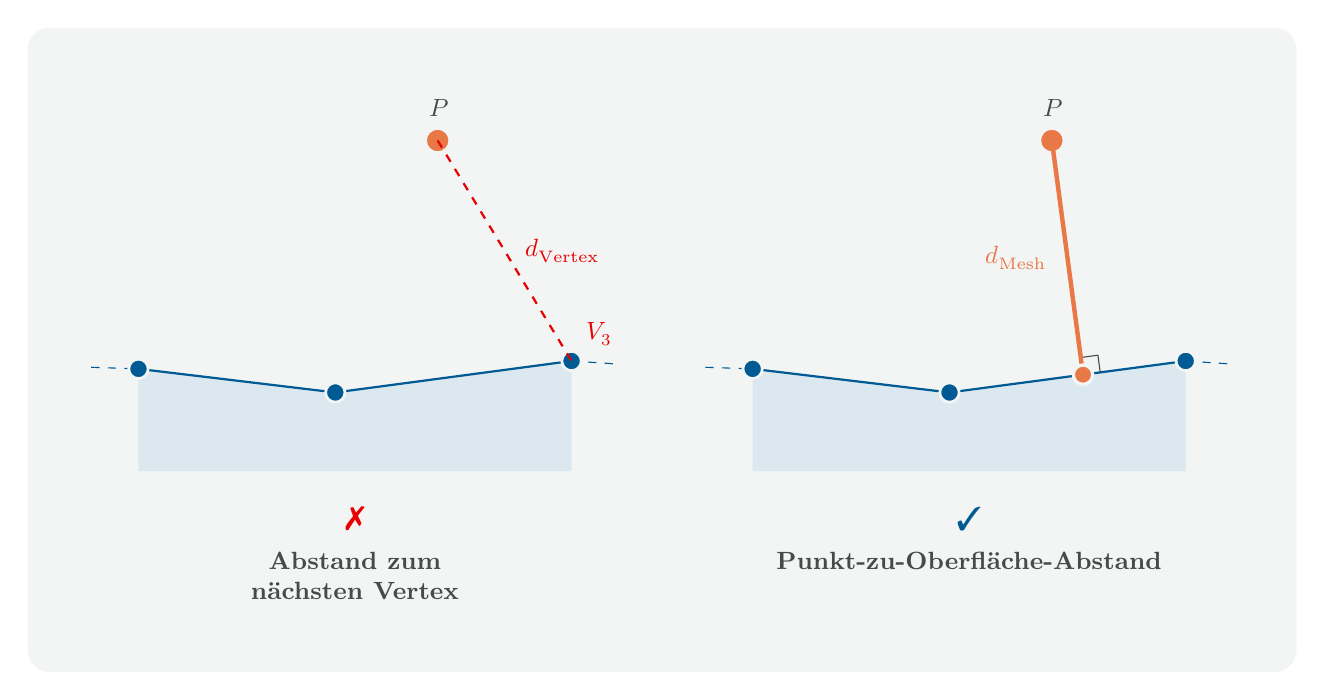
\begin{tikzpicture}[
    show background rectangle,
    background rectangle/.style={fill=my_lightgray, rounded corners=8pt},
    inner frame sep=0.8cm,
    annotation/.style={draw=my_darkgray, thick, -{Stealth[length=7pt, width=5pt]}}
]

% ======================================================
% Linkes Panel: naiver Abstand zum nächsten Vertex  (✗)
% ======================================================
\begin{scope}

  % Mesh-Fläche
  \fill[my_lightblue!70]
    (0,0.3) -- (2.5,0) -- (5.5,0.4) -- (5.5,-1.0) -- (0,-1.0) -- cycle;

  % Mesh-Kanten (gestrichelt an den Rändern = Fortsetzung des Netzes)
  \draw[my_darkblue, dashed, thin] (-0.6,0.32) -- (0,0.3);
  \draw[my_darkblue, thick]        (0,0.3) -- (2.5,0) -- (5.5,0.4);
  \draw[my_darkblue, dashed, thin] (5.5,0.4) -- (6.1,0.36);

  % Mesh-Vertices
  \foreach \x/\y in {0/0.3, 2.5/0, 5.5/0.4}{
    \filldraw[fill=my_darkblue, draw=my_lightgray, line width=1pt]
      (\x,\y) circle (3.5pt);
  }

  % Scan-Punkt P
  \filldraw[fill=my_orange, draw=my_lightgray, line width=1.2pt]
    (3.8,3.2) circle (4.5pt);
  \node[font=\small, text=my_darkgray, above=5pt] at (3.8,3.2) {$P$};

  % Linie zum nächsten Vertex V3=(5.5, 0.4)
  \draw[my_red, thick, dashed] (3.8,3.2) -- (5.5,0.4);

  % Label d_Vertex (mittig, rechts der Linie)
  \node[font=\small, text=my_red, right=4pt]
    at ($(3.8,3.2)!0.50!(5.5,0.4)$) {$d_{\mathrm{Vertex}}$};

  % Nächster Vertex V3 hervorheben
  \node[font=\small\bfseries, text=my_red, above right=2pt]
    at (5.5,0.4) {$V_3$};

  % Bewertungssymbol und Panel-Titel
  \node[font=\large\bfseries, text=my_red]
    at (2.75,-1.6) {\ding{55}};
  \node[font=\small\bfseries, text=my_darkgray, anchor=north, align=center]
    at (2.75,-1.9) {Abstand zum\\nächsten Vertex};

\end{scope}

% ======================================================
% Rechtes Panel: Punkt-zu-Oberfläche-Abstand  (✓)
% ======================================================
\begin{scope}[xshift=7.8cm]

  % Mesh-Fläche
  \fill[my_lightblue!70]
    (0,0.3) -- (2.5,0) -- (5.5,0.4) -- (5.5,-1.0) -- (0,-1.0) -- cycle;

  % Mesh-Kanten
  \draw[my_darkblue, dashed, thin] (-0.6,0.32) -- (0,0.3);
  \draw[my_darkblue, thick]        (0,0.3) -- (2.5,0) -- (5.5,0.4);
  \draw[my_darkblue, dashed, thin] (5.5,0.4) -- (6.1,0.36);

  % Mesh-Vertices
  \foreach \x/\y in {0/0.3, 2.5/0, 5.5/0.4}{
    \filldraw[fill=my_darkblue, draw=my_lightgray, line width=1pt]
      (\x,\y) circle (3.5pt);
  }

  % Scan-Punkt P
  \filldraw[fill=my_orange, draw=my_lightgray, line width=1.2pt]
    (3.8,3.2) circle (4.5pt);
  \node[font=\small, text=my_darkgray, above=5pt] at (3.8,3.2) {$P$};

  % Lotfußpunkt F=(4.196, 0.226) auf Kante V2-V3
  \coordinate (F) at (4.196, 0.226);

  % Rechter-Winkel-Marker bei F
  % Kantenrichtung  (unit): (0.991,  0.132)
  % Lotrichtung F->P (unit): (-0.132, 0.991)
  \draw[my_darkgray, thin]
    ($(F) + 0.22*(0.991,0.132)$) --
    ($(F) + 0.22*(0.991,0.132) + 0.22*(-0.132,0.991)$) --
    ($(F) + 0.22*(-0.132,0.991)$);

  % Senkrechte Linie (Lot) von P zu F
  \draw[my_orange, ultra thick] (3.8,3.2) -- (F);

  % Fußpunkt F markieren
  \filldraw[fill=my_orange, draw=my_lightgray, line width=1.2pt]
    (F) circle (3.5pt);

  % Label d_Mesh (mittig, links der Linie)
  \node[font=\small, text=my_orange, left=4pt]
    at ($(3.8,3.2)!0.50!(F)$) {$d_{\mathrm{Mesh}}$};

  % Bewertungssymbol und Panel-Titel
  \node[font=\large\bfseries, text=my_darkblue]
    at (2.75,-1.6) {\ding{51}};
  \node[font=\small\bfseries, text=my_darkgray, anchor=north, align=center]
    at (2.75,-1.9) {Punkt-zu-Oberfläche-Abstand};

\end{scope}

\end{tikzpicture}
\end{document}
